\section{实验}

\subsection{设置}

实验模型为Meta-Llama-3.1-8B-Instruct，source为已审计matched task group-scale hard checkpoint，逻辑码率约2.1207557 bpp。开放层为28--31，每层七个Linear（q/k/v/o/gate/up/down），共28个坐标。Assignment动作复用V14的固定curvature-ranked top-128 bundle；V15唯一新增动作是hard assignment后touched row/input group的闭式FP16 scale投影。实验不更换scorer、bundle、seed、group size、层序或文本阈值。

任务train包含ARC-C、ARC-E、HellaSwag、PIQA、WinoGrande各512条，共2560 examples、8193 choices、353058 tokens。Text train包含4096 sequences $\times$ 4096 tokens，共16,777,216 tokens。正式run使用当前本地服务器物理GPU4（A100-SXM4-80GB）单卡；未连接也未使用10.30.0.14。总耗时13,510.7063秒（3.7530小时），GPU peak memory为27,149,745,152 bytes（25.2852 GiB）。

\subsection{缓存与合同验证}

Task cache使用32个分层样本与同batch完整HF forward做parity，最大choice-score误差为$1.1444092\times10^{-5}$，32/32 argmax一致。Text prefix cache大小为
\begin{equation}
4096\times4096\times4096\times2=137{,}438{,}953{,}472\text{ bytes}=128\text{ GiB}.
\end{equation}
8个覆盖首尾位置的full-forward CE parity最大和平均误差均为0。Raw summary SHA256为\texttt{45e05f24b98bb677b10d25af2e06585195e026012aac3e91908b1f08342bd2d2}。程序正常退出，状态为\texttt{hard\_scale\_compensated\_gain\_rejected}；这表示方法gate失败，不是基础设施失败。

\subsection{主要结果}

\begin{figure*}[t]
\centering
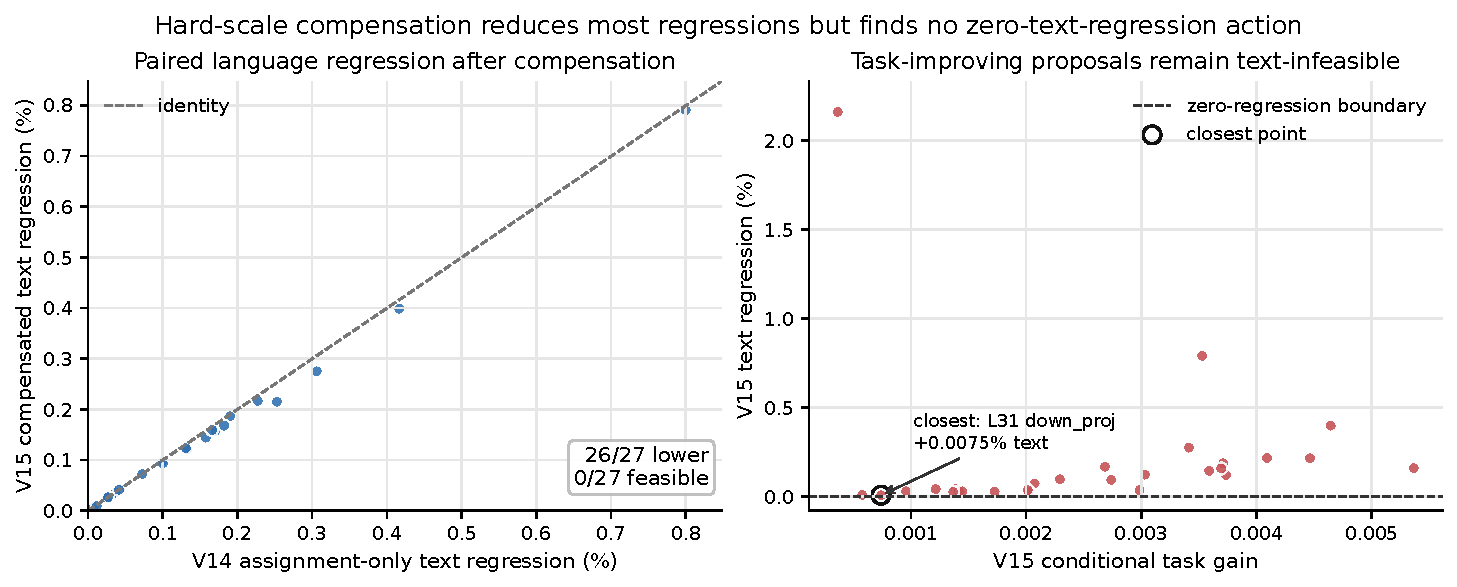
\includegraphics[width=0.94\textwidth]{../img/v15_compensation_feasibility.pdf}
\caption{Hard-first局部scale补偿的配对机制结果。左图只包含V14中task-improving且V15可匹配的27个共同坐标，其中26个的文本退化下降，但没有动作达到零退化。右图包含V15全部28个paired actions：它们都改善任务目标，却仍全部位于文本零退化边界之上。}
\label{fig:v15_compensation_feasibility}
\end{figure*}

\begin{table}[t]
\centering
\small
\caption{Hard-first local scale compensation的总体结果。}
\begin{tabular}{lr}
\toprule
指标 & 结果\\
\midrule
Paired candidates & 28\\
Task-improving & 28/28\\
Exact text-feasible & 0/28\\
Accepted bundles / switches & 0/0\\
Touched groups & 2,133\\
FP16后真实变化groups & 2,048\\
Weighted anchor error & 1.503737$\rightarrow$1.474448\\
Weighted anchor error降幅 & 1.9477\%\\
最大单group相对scale变化 & 31.4247\%\\
\bottomrule
\end{tabular}
\end{table}

Source task balanced combined loss为0.3297837665，source text CE为2.1035536536。28个paired actions全部降低task-train loss，但28个动作的完整text CE全部高于source，因此text-feasible数量为0，accepted bundles/switches为0/0。由于没有非零endpoint，task validation、text validation、task audit、text audit、checkpoint、WikiText2 PPL与lm\_eval均未访问。

\begin{table}[t]
\centering
\small
\caption{每层最接近零文本退化的paired action。}
\begin{tabular}{rllrr}
\toprule
Layer & 坐标 & Task gain & Text CE相对退化 & 可行\\
\midrule
28 & mlp.down\_proj & 0.0009583 & +0.0296650\% & 否\\
29 & self\_attn.o\_proj & 0.0014160 & +0.0289287\% & 否\\
30 & mlp.down\_proj & 0.0020233 & +0.0259710\% & 否\\
31 & mlp.down\_proj & 0.0007411 & +0.0074999\% & 否\\
\bottomrule
\end{tabular}
\end{table}

最大任务收益来自layer-30 \texttt{mlp.up\_proj}：combined loss下降0.0053658，但text CE增加0.1593725\%。最大文本退化来自layer-29 \texttt{self\_attn.q\_proj}：text CE增加2.160956\%，任务收益仅0.0003638。

``Local''只描述支持集。为避免把它误读为小幅更新，我们统计28个动作各自的组内最大相对scale变化：中位数为5.0238\%，nearest-rank p90/p95分别为16.5939\%/18.2663\%，最大值为31.4247\%。原始summary没有持久化2,133个group的逐组变化，因而这些不是group-level分位数；完整逐组分布是当前证据的复现限制。

\subsection{与assignment-only的机制对比}

V15的负结果不能简单解释为scale补偿无效。与V14 assignment-only的27个共同坐标相比，V15在26/27个动作上降低文本退化，只有layer-30 \texttt{self\_attn.o\_proj}轻微变差。平均变化为-0.0072663 percentage points。最大改善来自layer-28 \texttt{self\_attn.k\_proj}，文本退化从0.2528836\%降到0.2153255\%。最接近可行的layer-31 \texttt{mlp.down\_proj}从0.0078526\%降到0.0074999\%。

如图~\ref{fig:v15_compensation_feasibility}所示，hard-first compensation捕捉到了真实的幅值修复信号：它降低局部hard-weight扰动，也几乎一致降低文本代价。但它没有改变可行性拓扑：连续的幅值改善没有让任何点跨过零退化边界。换言之，V14的冲突不只是“assignment变了，scale没动”；还存在单个group乘性scale无法修复的方向误差、跨Linear传播或residual-stream耦合。

方法演进进一步排除了两个更简单解释：V9的soft joint scale--assignment在hard projection后失配，说明补偿必须作用于真实离散态；V14的assignment-only搜索得到0/27可行，说明固定scale的动作空间不足；V15修复前者并扩展后者，却仍得到0/28可行。因此，当前证据将瓶颈从soft--hard交接和纯幅值失配推进到方向性与跨模块传播，但尚未验证何种更高维补偿能够产生端点。

\begin{table*}[t]
\centering
\small
\caption{从V8到V15的机制梯级。V15只排除自然的局部幅值解释，不证明所有assignment全局不可行。}
\begin{tabular}{llll}
\toprule
版本 & 机制问题 & 正式结果 & 被排除的简单解释\\
\midrule
V8 & Scale-only与assignment-only是否近似等价 & Scale更强，assignment漂移较小 & 二者并非等价坐标\\
V9 & Soft joint是否产生互补 & Joint被scale-only严格支配 & Soft补偿不能直接交给hard投影\\
V14 & Assignment-only是否有零退化任务收益 & 27个task gain，0个feasible & 固定assignment-only空间为空\\
V15 & Hard-first scale repair是否打开可行域 & 28个task gain，0个feasible & 简单局部幅值补偿不足\\
\bottomrule
\end{tabular}
\end{table*}

\subsection{边界与不能声称的内容}

本文没有产生deployable endpoint，因此不能报告新的PPL/accuracy，也不能声称超过QTIP、GSQ或source。0/28可行只适用于当前Llama-3.1-8B-Instruct、最后四层、固定top-128 bundle、完整text-train零退化合同和hard-first local scale compensation。它不证明所有VQ assignment全局不可行，也不否认非零文本预算、跨层补偿、低秩残差或重新设计的候选动作可能有效。

同样，V15不是一个调参实验。它没有扫描group size、bundle size、seed、scale clipping或文本预算；这些扫描即使找到更好点，也会回答不同问题。本文回答的是：在最小新增自由度“touched group的闭式幅值补偿”下，原先空的零退化可行域是否变为非空。正式答案是否定的。
